% 12 variables in here:
% H_1 = 10.0, H_2 = 10.0, H_3 = 10.0, U_1 = 0.0, U_2 = 0.0, U_3 = 0.0, h_1 = 10.0, h_2 = 10.0, h_3 = 10.0, u_1 = 0.0, u_2 = 0.0, u_3 = 0.0
\begin{figure}[h!]
  \centering
  % \quad \subfloat[] {
  % 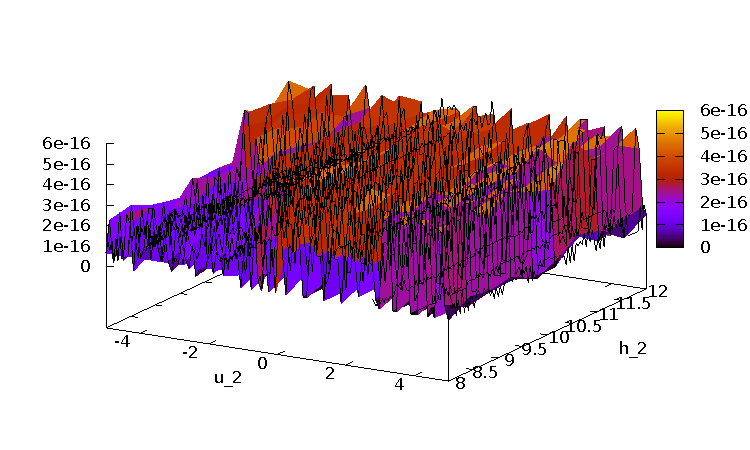
\includegraphics[scale=\zoomfactor]{{{equidist_2_default/10.0_10.0_0.0_0.0_10.0_y_0.0_xf00}}}
  % }
  % \quad \subfloat[] {
  % 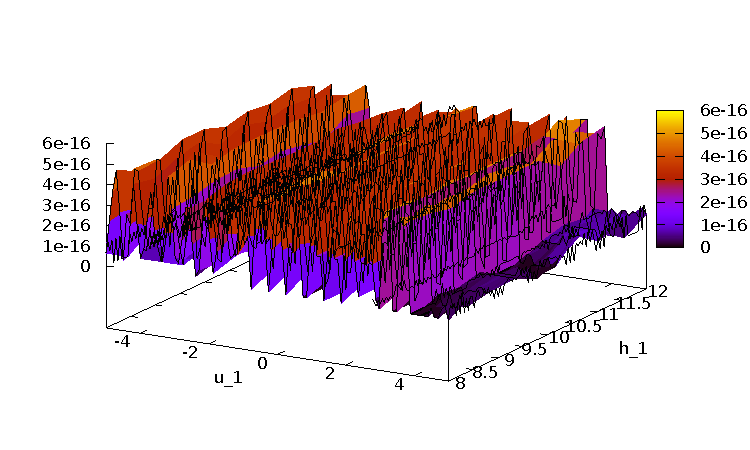
\includegraphics[scale=\zoomfactor]{{{equidist_2_default/10.0_10.0_0.0_0.0_y_10.0_x_0.0f00}}}
  % }
  \quad \subfloat[Momentum error for $p_1^L$ resp. $p_2^L$ if we use support points $\{0,1\}$] {
    \begin{tikzpicture}
      \node at (0,0) {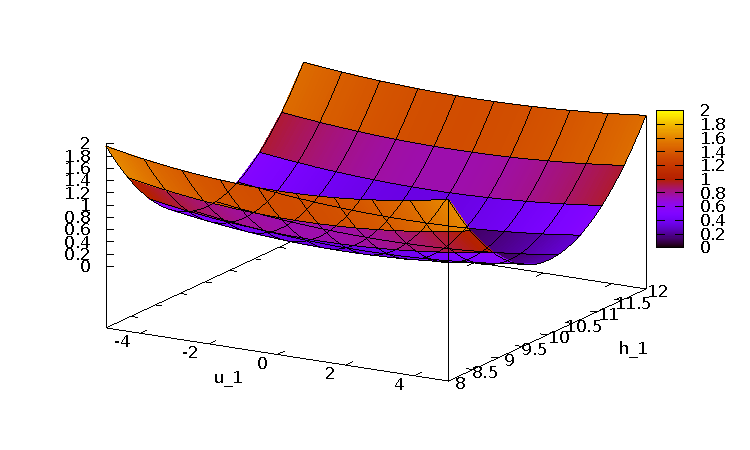
\includegraphics[scale=\zoomfactor]{{{equidist_2_default/10.0_10.0_0.0_0.0_y_10.0_x_0.0f01}}}};
      \node[align=right, text width=3cm] at (.2,1.33) {\textsf{\tiny{Momentum error}}};
      \draw(1.8,1.34)-- +(.4cm,0);
    \end{tikzpicture}
  }
  \hspace{.3cm}
  % \quad \subfloat[Momentum error for $p_2^L$ if we use support points $\{0,1\}$] {
  %   \begin{tikzpicture}
  %     \node at (0,0) {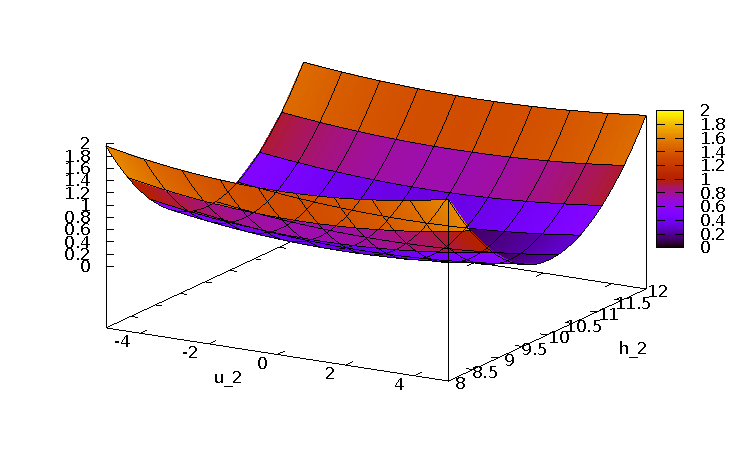
\includegraphics[scale=\zoomfactor]{{{equidist_2_default/10.0_10.0_0.0_0.0_10.0_y_0.0_xf01}}}};
  %     \node[align=right, text width=3cm] at (.2,1.33) {\textsf{\tiny{Momentum error}}};
  %     \draw(1.8,1.34)-- +(.4cm,0);
  %   \end{tikzpicture}
  % }
  \quad \subfloat[Momentum error for $p_1^L$ resp. $p_2^L$ if we use support points $\{0.5\pm\frac{\sqrt{3}}{6}\}$]{
    \begin{tikzpicture}
      \node at (0,0) {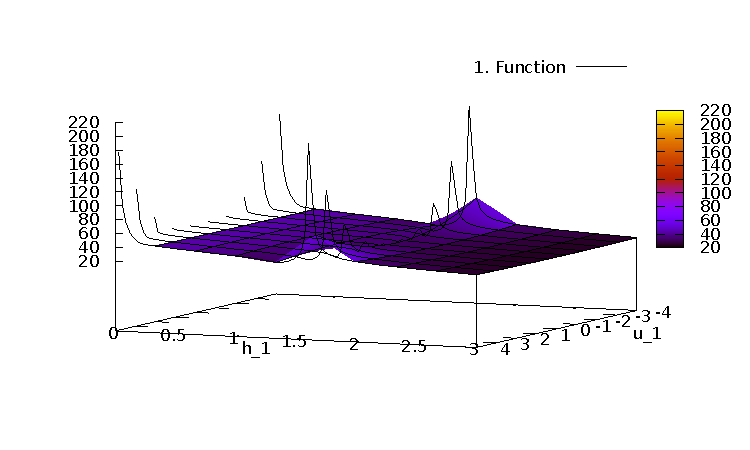
\includegraphics[scale=\zoomfactor]{{{2_punkte_alles_10_0/x_y_0.0_10.0_0.0_10.0_0.0_10.0f1}}}};
      \fill[white] (.8,1.2) rectangle (1.75,1.5);
      \node[align=right, text width=3cm] at (.2,1.33) {\textsf{\tiny{Momentum error}}};
    \end{tikzpicture}
  }
  % \hspace{.3cm}
  % \quad \subfloat[Momentum error for $p_2^L$ if we use support points $\{0.5\pm\frac{\sqrt{3}}{6}\}$]{
  %   \begin{tikzpicture}
  %     \node at (0,0) {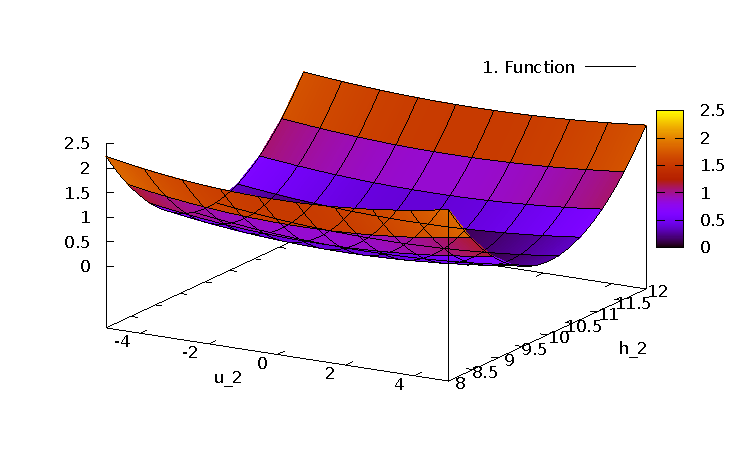
\includegraphics[scale=\zoomfactor]{{{2_punkte_alles_10_0/0.0_10.0_0.0_10.0_x_y_0.0_10.0f1}}}};
  %     \fill[white] (.8,1.2) rectangle (1.75,1.5);
  %     \node[align=right, text width=3cm] at (.2,1.33) {\textsf{\tiny{Momentum error}}};
  %   \end{tikzpicture}
  % }
  \caption{Momentum errors for two support points per edge. We compare different settings of support points (support points at 0 and 1 vs. support points as used in Gaussian quadrature). All support points are set to $(10,0)^T$.}
  \label{fig:equidist_2_default}
\end{figure}

%%% Local Variables:
%%% TeX-master: "../results.tex"
%%% End:
